\documentclass[12pt]{article}
\usepackage[utf8]{inputenc}
\usepackage{graphicx}

\usepackage{hyperref}
\hypersetup{hypertex=true,
            colorlinks=true,
            linkcolor=red,
            anchorcolor=red,
            citecolor=red}
            
\usepackage[section]{placeins}
\usepackage{float}
\usepackage{xcolor}
\usepackage{appendix}
\usepackage{blindtext}
\usepackage[textwidth=14.5cm]{geometry}
\usepackage{listings}
\lstset{
 columns=fixed,       
 numbers=left,                                        % 在左侧显示行号
 numberstyle=\tiny\color{gray},                       % 设定行号格式
 frame=none,                                          % 不显示背景边框
 backgroundcolor=\color[RGB]{245,245,244},            % 设定背景颜色
 keywordstyle=\color[RGB]{40,40,255},                 % 设定关键字颜色
 numberstyle=\footnotesize\color{darkgray},           
 commentstyle=\it\color[RGB]{0,96,96},                % 设置代码注释的格式
 stringstyle=\rmfamily\slshape\color[RGB]{128,0,0},   % 设置字符串格式
 showstringspaces=false,                              % 不显示字符串中的空格
 %title=\lstname                                      % 设置语言
}
\usepackage{amsmath}
\numberwithin{figure}{subsection}
\numberwithin{table}{subsection}
\usepackage{caption}
\captionsetup[figure]{labelfont={bf},
                      labelformat={default},
                      labelsep=period,name={Figure.}
                      }
\captionsetup[table]{labelfont={bf},
                      labelformat={default},
                      labelsep=period,name={Table.}
                      }

\graphicspath{{images/}}

\begin{document}
\title{\textbf{Project in ME001 -- Sampling system\\Group 1}}

\author{By Chen YuXuan 1809853J-I011-0011 D1\\ \\
Wang Yuan 1809853G-I011-0030 D1\\ \\
He PeiLin 1809853U-I011-0078 D1}

\date{December 2, 2020}
\maketitle

\newpage
\tableofcontents
\newpage

\section{Restatement of the Problem}
In this project, we are expected to extract a subset of samples of big data. Assume there are $m$ samples ($45\leq m\leq54$), 
any $n$ ($7 \leq n\leq 25$) samples out of these m samples are selected. 
There are $C_{n}^{m}$ groups of $n$ samples. From one of these groups of n samples, we randomly selected $k$ ($4 \leq k \leq 7$) samples to form some groups. 
So there will be $C_{n}^{k}$ groups of k samples selected. There are at least \textbf{ONE} group of k samples, 
in which $s$ ($3 \leq s \leq 7$) samples have been selected from the $j$ (where $s \leq j \leq k$) samples.
Among these groups of $k$ samples, we would like to optimize them by selecting ONLY some of them.

 

\section{Basic Ideas}

We can divide the probelm into two parts, $j=s$ and $j \neq s$.
\subsection{$j=s$}
    \begin{enumerate}
        \item \textbf{Lemma one: Algorithm to Find Subsets}
        Now, we have a set whose number of the element is $n$. Then we want to find out all the subsets whose 
        number of the element is $k$.\\
        \textbf{Algorithm: \\}
        \begin{itemize}
            \item First, we put the orign set to a container, and then we label every element to one(illustrate the picture below). 
            We assume that the orign set is $S$, $S=\{1,2,3,4,5\}$:\\
            \begin{table}[H]
            \centering
            \begin{tabular}{lllll}
            \hline
            \multicolumn{1}{|l|}{5} & \multicolumn{1}{l|}{4} & \multicolumn{1}{l|}{3} & \multicolumn{1}{l|}{2} & \multicolumn{1}{l|}{1} \\ \hline
            1                       & 1                      & 1                      & 1                      & 1                     
            \end{tabular}
            \end{table}
            Then, the subset which has the same element with the orignal set's, I'll label the element to 1, otherwise I'll label it to 0. For 
            example, we suppose that one the subset is $S_1$,$S_1=\{1,2,4\}$. We can represent it as below:\\
            \begin{table}[H]
            \centering
            \begin{tabular}{lllll}
            \hline
            \multicolumn{1}{|l|}{5} & \multicolumn{1}{l|}{4} & \multicolumn{1}{l|}{3} & \multicolumn{1}{l|}{2} & \multicolumn{1}{l|}{1} \\ \hline
            0                       & 1                      & 0                      & 1                      & 1                     
            \end{tabular}
            \end{table}
            Now we can change the number below the array to a binary number, which means that each subset can be represented by a unique number from 
            0(empty set) to $2^n-1$(orignal set). Just like the example above set $S$ can be represented by $11111_2 = 31_{10}$ and $S_1$ can be expressed 
            as $01011_2 = 11_{10}$
            \item Now, we know how to find subsets of the original set, but I want to know how to find the subset with the specific number of elements. 
            Therefore, we only need to know the subset whose binary number representation contains $k$ 1s. As the example above, $S_1=\{1,2,4\}$:
            \begin{table}[H]
            \centering
            \begin{tabular}{lllll}
            \hline
            \multicolumn{1}{|l|}{5} & \multicolumn{1}{l|}{4} & \multicolumn{1}{l|}{3} & \multicolumn{1}{l|}{2} & \multicolumn{1}{l|}{1} \\ \hline
            0                       & 1                      & 0                      & 1                      & 1                     
            \end{tabular}
            \end{table}
            So, the $S_1$ contains three elements, because it has three 1s.\\
            In this way, we can easily find out the subset whose number of elements is k from $0$ to $2^n-1$, the code illustrates below:
\begin{lstlisting}
void findSubsetOfk(int n,int k, vector<int> subsetK){
    int count=0;//number of 1s
    for(int i = 1 ; i < (1<<n); i++){
        for(int j = 0; j < n; j++){
            //the binary number representation 
            //of subset has an 1 on the jth position
            if(i & (1<<j)!=0){
                count++;
            }
        }
        if(count==k)
            susetK.empalce_back(i);
        count=0;
    }

}
\end{lstlisting}
        But,we can easily find that the binary number representation of the subset whose number of elements is k is 
        no less than $2^k-1$. Therefore, we the code above, we can have an optimization on the i. THe optimized code is 
        below:\\
\begin{lstlisting}
void findSubsetOfk(int n,int k, vector<int> subsetK){
    int count=0;//number of 1s
    for(int i = (1<<k)-1 ; i < (1<<n); i++){
        for(int j = 0; j < n; j++){
            //the binary number representation 
            //of subset has an 1 on the jth position
            if(i & (1<<j)!=0){
                count++;
            }
        }
        if(count==k)
            susetK.empalce_back(i);
        count=0;
    }

}
\end{lstlisting}
        \end{itemize}
        \begin{itemize}
            \item Currently, we can use the same way what we say above to find out the subset of the set whose number of element is 
            $k$ and its number of elements is $s$.
        \end{itemize}
    \item \textbf{Lemma two: Calculate the Combination number}\\
    If we calculate the combination number directly, it is likely to out of bounds of int. So we can use this combination formula below:
    $$C_n^m=C_{n-1}^{m-1}+C_{n-1}^m$$
    to calculate the combination number. The code is below:
\begin{lstlisting}
int calculateCombinationNumber(int n,int m){
    for(int i=0;i<=n;i++)
        C[i][0]=1;
    for(int i=1;i<=n;i++)
        for(int j=1;j<=i;j++)
            C[i][j]=C[i-1][j-1]+C[i-1][j];
    return C[n][m];
}
\end{lstlisting}
    \item \textbf{Lemma three: Greedy algorithm to calculate the set covergae}\\
    We denote that the input is a set $\mathcal{U}$ of n elements, and a collection $S=\{S_1, S_2, . . . , S_m\}$ of $m$ subsets of $\mathcal{U}$ such that
    $\cup_iS_i=\mathcal{U}$. Our goal is to take as few subsets as possible from $S$ such that their union covers $\mathcal{U}$.
    We can solve this problem easily by greedy algorithm. The algorithm is below:
    \begin{table}[H]
        \centering
        \begin{tabular}{|l|}
        \hline
        Greedy Cover($S$,$\mathcal{U}$)                                                     \\
        1. repeat                                                             \\
        2.     pick the set that covers the maximum number of uncover element \\
        3.     mark elements in the chosen set as covered                     \\
        4.     remove the set from $S$ to the result set                        \\
        5. done                                                               \\ \hline
        \end{tabular}
        \end{table}
    \end{enumerate}
    Based on the three lemmas above, we can easily transform the problem to that the set $\mathcal{U}=\{1,2,\cdots, C^j_n\}$, which means that we map each different subset 
    whose the number of the elements is j to a unique code from 1 to $ C^j_n$. Each subset of $S$, represents the each $k$ set's subsets whose number of elements is j. Ultimately, 
    we can solve the problem easily.
\subsection{$j \neq s$}
    The way to solve the problem is just like the way we mentioned above. However, after finishing finding the subset of the $k$ set whose element number is $s$, we should know how many sets 
    whose the number of elements is $j$ include it. Therefore, we use dfs(depth first search) to find out them.
    Assuming that $n=5, s=3, j=4$, and the subset whose number of elements is equal to 3 is labeled as $01011_2$. Therefore, we can expand it as below:
    \begin{table}[H]
        \centering
        \begin{tabular}{lllll}
        \hline
        \multicolumn{1}{|l|}{5} & \multicolumn{1}{l|}{4} & \multicolumn{1}{l|}{3} & \multicolumn{1}{l|}{2} & \multicolumn{1}{l|}{1} \\ \hline
        0                       & 1                      & 0                      & 1                      & 1                      \\
        0                       & 1                      & 1                      & 1                      & 1                      \\
        1                       & 1                      & 0                      & 1                      & 1                     
        \end{tabular}
        \end{table}
    Then, we should mark the last two rows of the set above in the $\mathcal{U}$ as covered.

\section{Essential Codes and Functions Analysis}
\subsection{Realization of Modifying DB files}

As the request said, we need output the group of $k$ samples and corresponding result in DB files.
Consequently, the OOP program language \textbf{C\#} can provide abundant libraries
to help realize combine with modifying DB files.

Depending on \textbf{C\#} powerful library and interface, we can apply our algorithm source code on GUI platform,
and realize the operation of creating new files(Code.\hyperref[code:create]{1}), 
exporting result into corresponding files(Code.\hyperref[code:insert]{2})
as well as deleting the specular data(Code.\hyperref[code:delete]{3}).  
\label{code:create}\lstinputlisting[language=c++]{code/createTable.cs}
\label{code:insert}\lstinputlisting[language=c++]{code/insertTable.cs}
\label{code:delete}\lstinputlisting[language=c++]{code/deleteTable.cs}
\subsection{Multi-Threading}
    
We adopt multi-threading programming way. We split the program into two parts, which are the GUI part and the 
calculation part. In this way, even if the program haven't figured out, the window of the program won't be stick.
The specific implemented function is bound in \hyperref[code:multi]{button2\_Click}.
\label{code:multi}\lstinputlisting[language=csh]{code/threading.cs}

    


\section{Steps to Run the Program}
In order to make the operation more smooth, all the program environment and settings are completed and included in the file package. Just required to follow the steps below to run the program.
\begin{enumerate}

\item Open the package and find the Information System Project.exe file. Double-click the file to enter the program interface as below exactly.
\begin{center}
    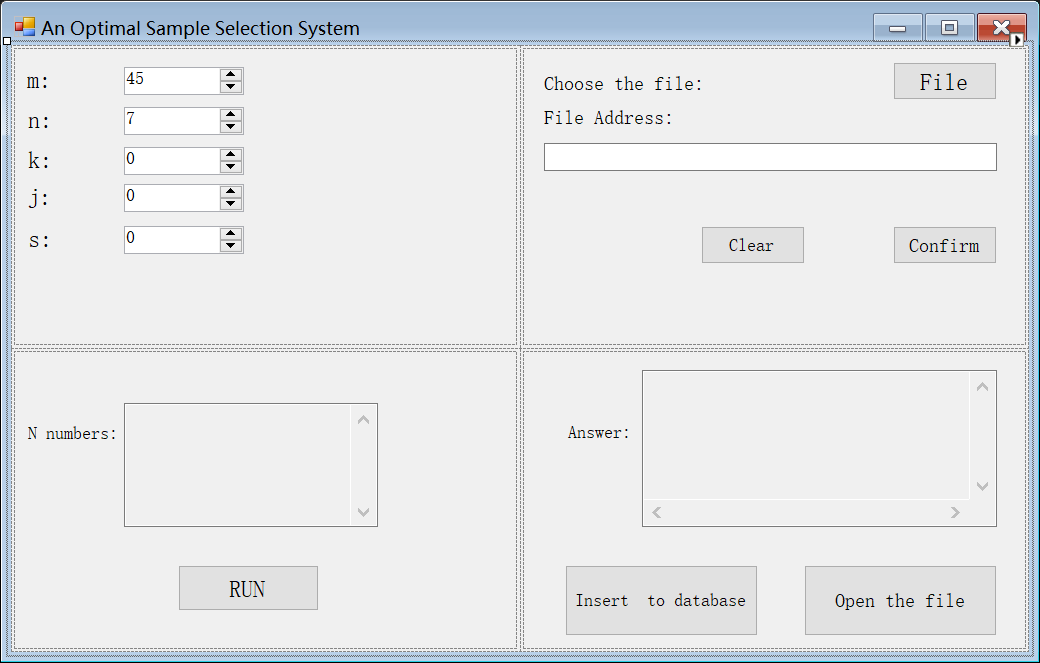
\includegraphics[width=10cm,height=6cm]{images/initial.png}
\end{center}

\item In order to record the relevant output data of the program and facilitate display and modification later. It is required to have a .mdb file to store it, which is called ---.mdb in project package.

\item Choose the data of each parameter and input on the program surface.
\begin{center}
    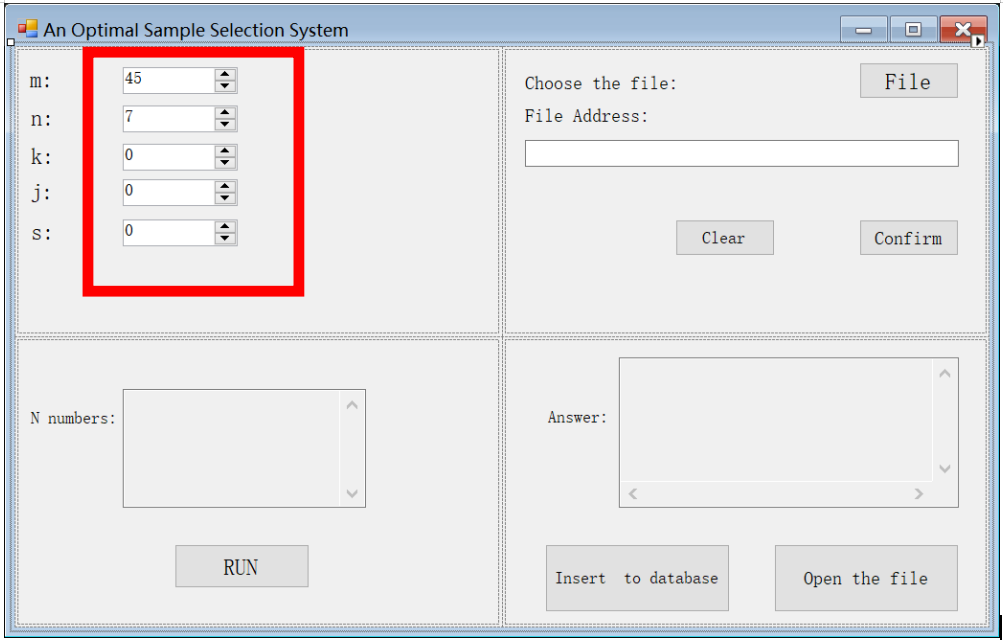
\includegraphics[width=10cm,height=6cm]{images/step1.PNG}
\end{center}

\item Choose the DB file to store and operate the data, click the 'File' and choose the ---.mdb in the previous step and 'Confirm' if all get right.(\textit{'clear' is a function that clear all the data you have input, include the parameter in step 3})
\begin{center}
    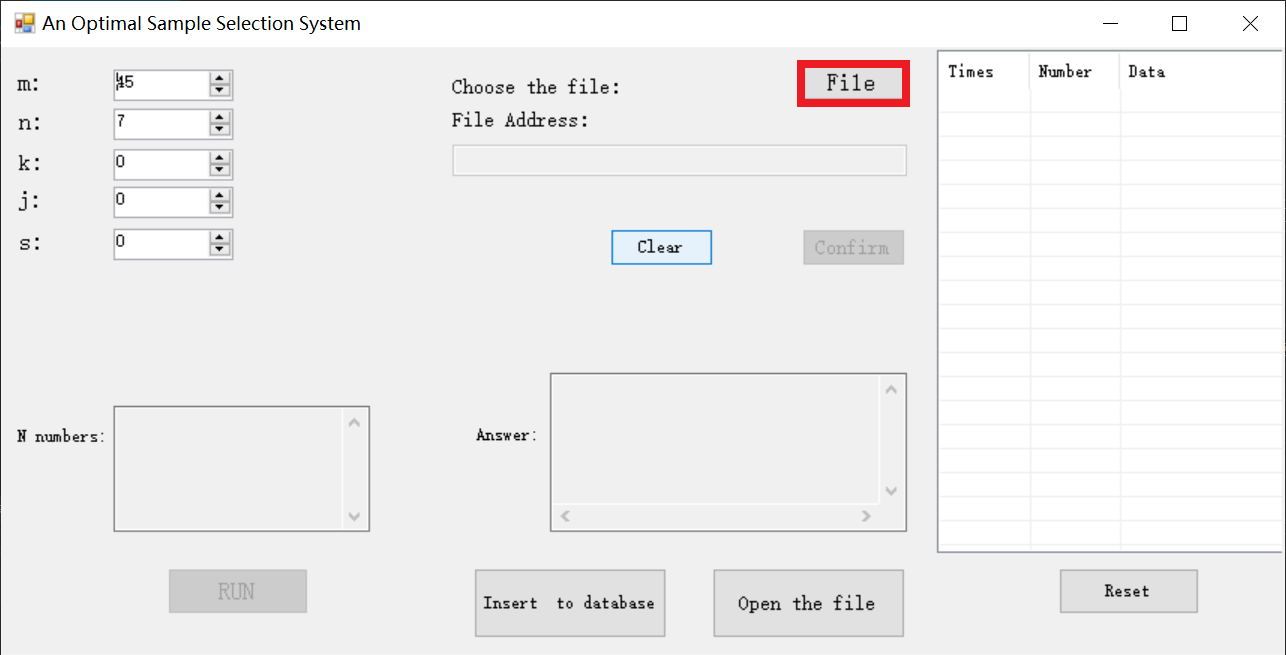
\includegraphics[width=10cm,height=6cm]{images/step2.PNG}
\end{center}
\begin{center}
    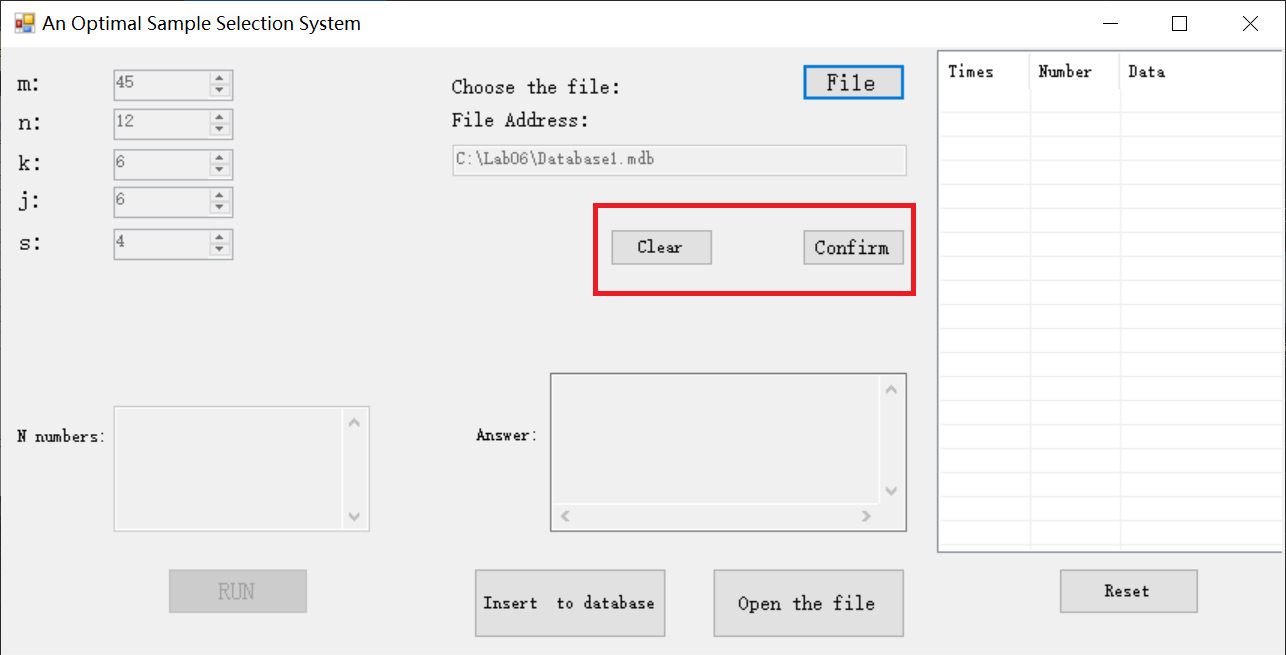
\includegraphics[width=10cm,height=6cm]{images/step3.PNG}
\end{center}

\item Push the 'RUN' button and the N number and final answer of your input will be shown on the surface window, you can check the answer after that.
\begin{center}
    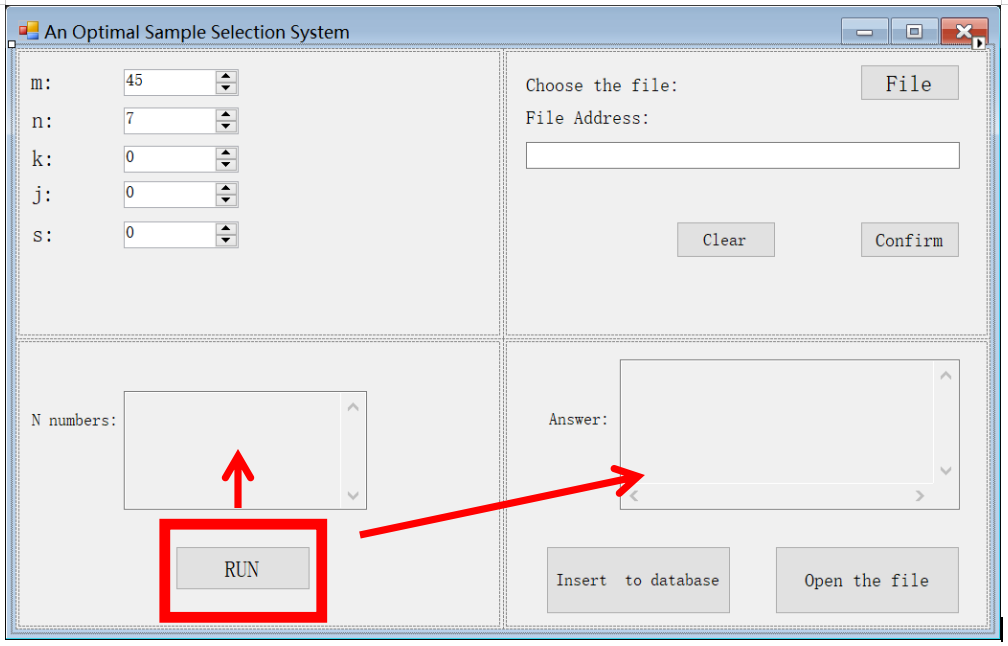
\includegraphics[width=10cm,height=6cm]{images/step4.PNG}
\end{center}

\item After confirm the data is correct, use 'Insert to database' to download the data on the DB file(---.mdb), and 'Open the file' can open it to display the data you have calculate. It is also easy for you to delete or use any other operation on the data though your DB file.
\begin{center}
    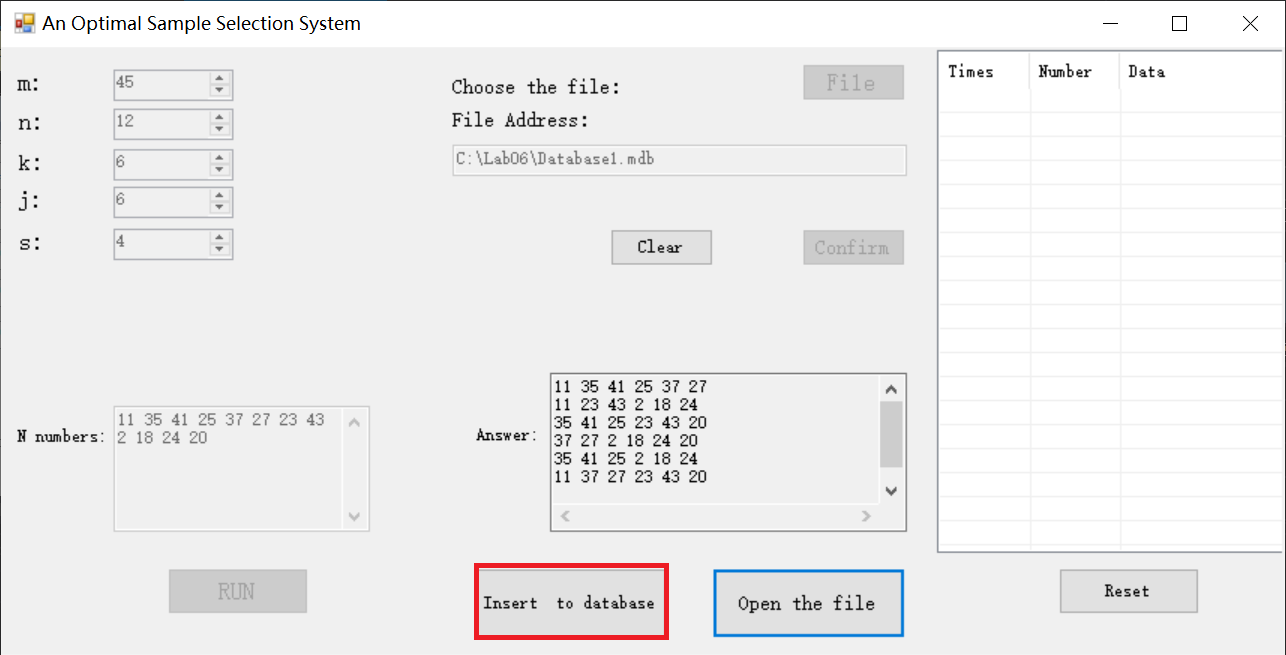
\includegraphics[width=10cm,height=6cm]{images/step5.PNG}
\end{center}
\begin{center}
    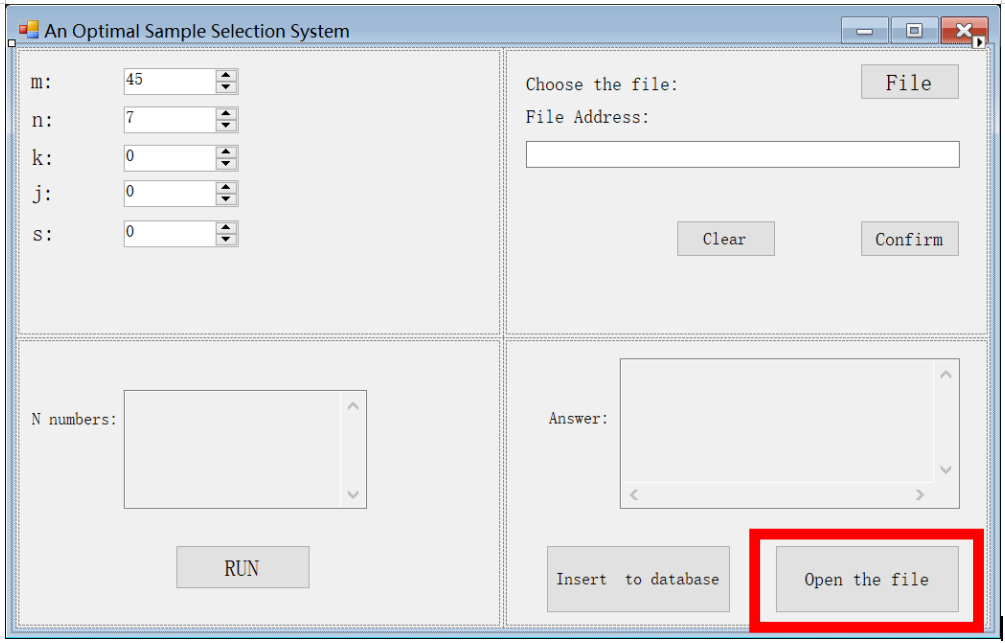
\includegraphics[width=10cm,height=6cm]{images/step6.PNG}
\end{center}

\end{enumerate}

\section{Program Test}
If the program window can be displayed normally, you can enter the value for verification. The conditions of 1, 2, 3 and 4, 5 and 6, 7 in the project requirement file are similar, so we choose 1, 4, and 6 as the demo of our program.
\begin{itemize}
\item E.g.$1$: Input the data: $m=45, n=7, k=6, j=5, s=5.$
\begin{center}
    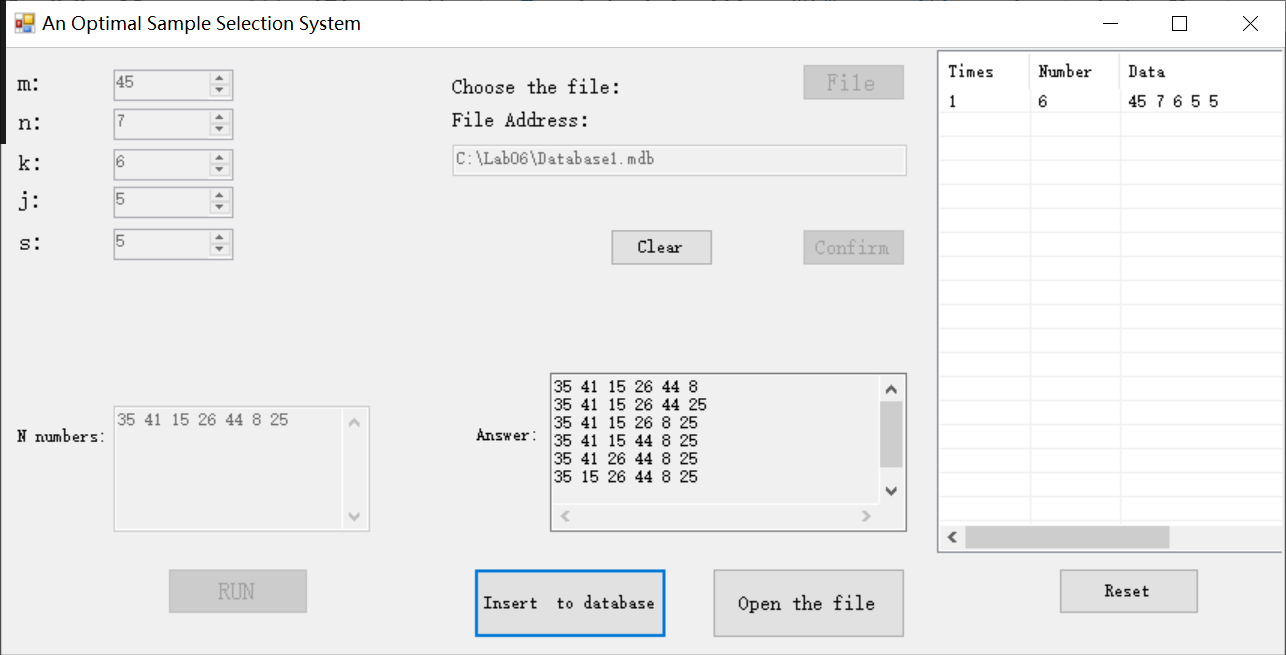
\includegraphics[width=10cm,height=6cm]{images/1.png}
\end{center}

\item E.g.$4$: Input the data: $m=45, n=8, k=6, j=6, s=5.$
\begin{center}
    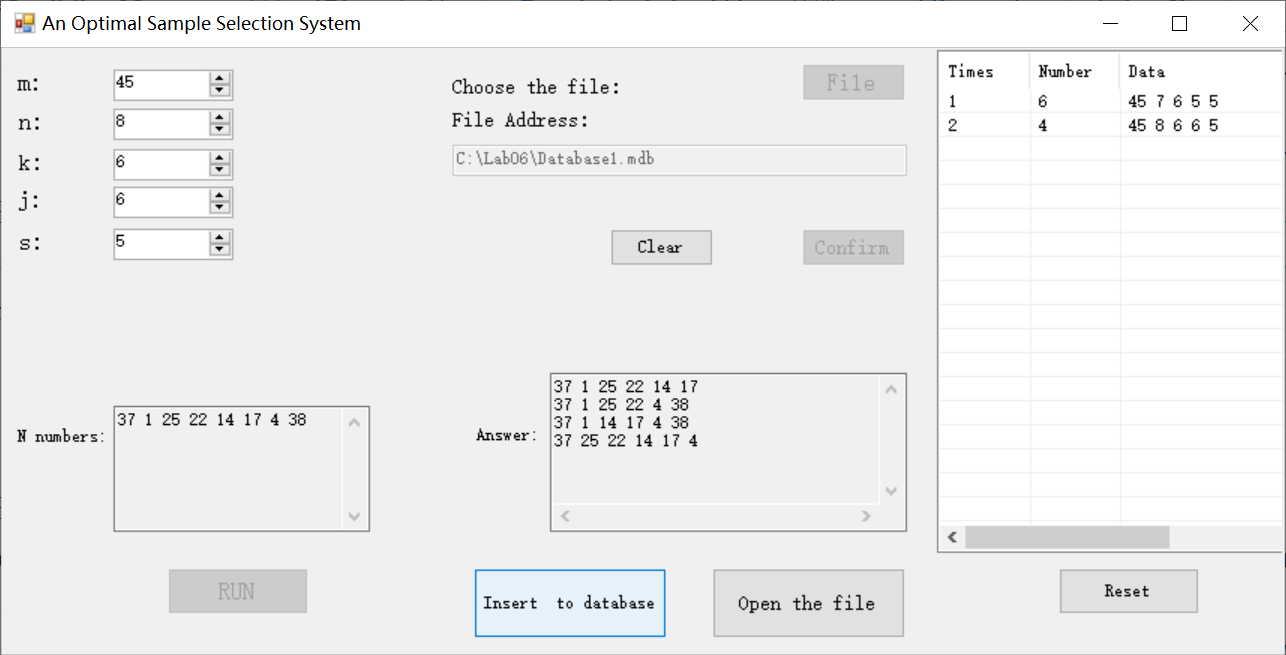
\includegraphics[width=10cm,height=6cm]{images/4.png}
\end{center}

\item E.g.$6$: Input the data: $m=45, n=10, k=6, j=6, s=4.$
\begin{center}
    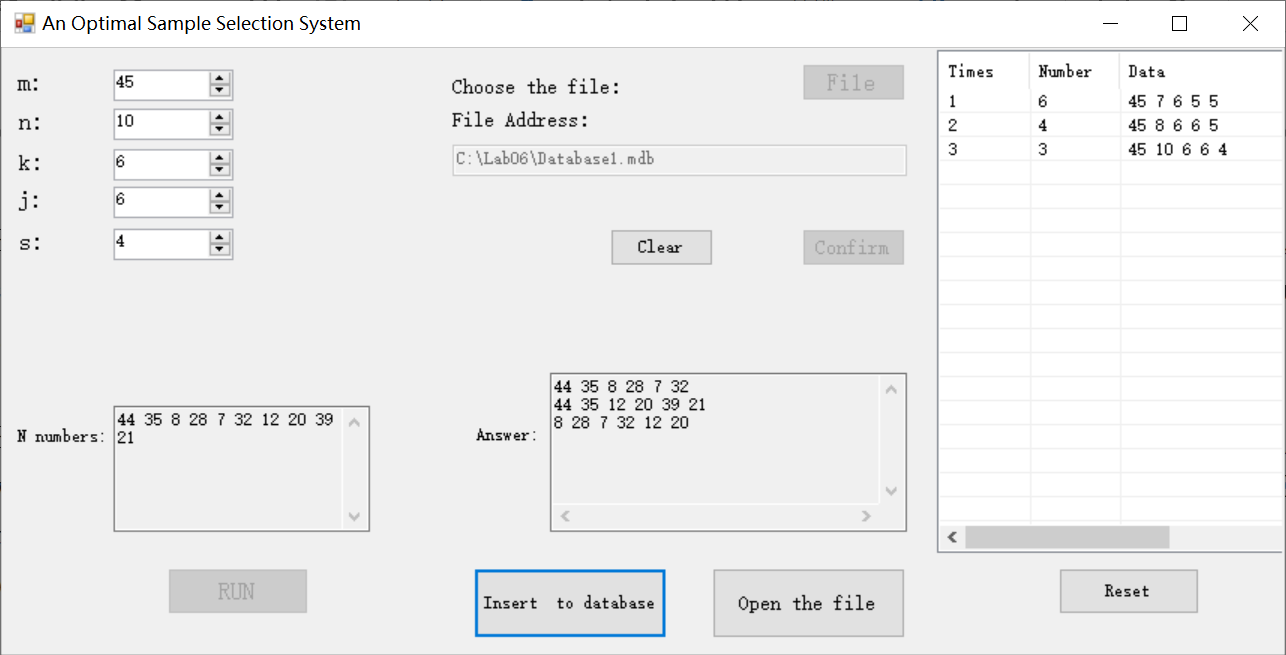
\includegraphics[width=10cm,height=6cm]{images/6.png}
\end{center}

\end{itemize}



\section{Summary}
This project is based on the theoretical direction of \textbf{ME001} subject and 
combines some knowledge of data structure and mathematic, 
including optimal algorithms and combinatorics. But there are no correct understanding of 
some part of difficult and profound mathematic problems like fuzzy set.
Authors point out about converse decimal digits to the binary make the big data abstraction in order to descend the time complexity.
By using program, authors realize the process from theory to practice reflecting the theoretical view of unity of knowledge and practice.
When writing large-scale projects, people often need cooperation and collaborative development, 
authors use \textbf{GitHub} for collaborative development and submit own patch code to collaborator's repository.
In this article, we will utilize ideas to achieve team cooperation on \textbf{GitHub}.
The last but not least, the goal of the future study and work is to work harder to learn this knowledge, 
in order to enrich, improve our level.


\bibliographystyle{plain}
\bibliography{}
\newpage
\appendix
\appendixpage
\addappheadtotoc
    \section{Programs for Algorithms}
        \lstset{title=\lstname}
        \lstinputlisting[language=c++]{source/Algorithm.cs}
    \section{Programs for GUI}
        \lstset{title=\lstname}
        \lstinputlisting[language=c++]{source/Form1.cs}
\end{document}
